\documentclass[a4paper,12pt,twoside,openany]{report}
%
% Wzorzec pracy dyplomowej
% J. Starzynski (jstar@iem.pw.edu.pl) na podstawie pracy dyplomowej
% mgr. inż. Błażeja Wincenciaka
% Wersja 0.1 - 8 października 2016
%
\usepackage{polski}
\usepackage{helvet}
\usepackage[T1]{fontenc}
\usepackage{anyfontsize}
\usepackage[utf8]{inputenc}
\usepackage[pdftex]{graphicx}
\usepackage{tabularx}
\usepackage{array}
\usepackage[polish]{babel}
\usepackage{subfigure}
\usepackage{amsfonts}
\usepackage{verbatim}
\usepackage{indentfirst}
\usepackage[pdftex]{hyperref}


% rozmaite polecenia pomocnicze
% gdzie rysunki?
\graphicspath{ {rys/} }
% oznaczenie rzeczy do zrobienia/poprawienia
\newcommand{\TODO}{\textbf{TODO}}


% wyroznienie slow kluczowych
\newcommand{\tech}{\texttt}

% na oprawe (1.0cm - 0.7cm)*2 = 0.6cm
% na oprawe (1.1cm - 0.7cm)*2 = 0.8cm
%  oddsidemargin lewy margines na nieparzystych stronach
% evensidemargin lewy margines na parzystych stronach
\def\oprawa{1.05cm}
\addtolength{\oddsidemargin}{\oprawa}
\addtolength{\evensidemargin}{-\oprawa}

% table span multirows
\usepackage{multirow}
\usepackage{enumitem}    % enumitem.pdf
\setlist{listparindent=\parindent, parsep=\parskip} % potrzebuje enumitem

%%%%%%%%%%%%%%% Dodatkowe Pakiety %%%%%%%%%%%%%%%%%
\usepackage{prmag2017}   % definiuje komendy opieku,nrindeksu, rodzaj pracy, ...
\usepackage{xspace}

%%%%%%%%%%%%%%% Strona Tytułowa %%%%%%%%%%%%%%%%%
% To trzeba wypelnic swoimi danymi
\title{Aplikacja do rozpoznawania emocji w sygnale mowy}

% autor
\author{Wojciech Decker}
\nrindeksu{252545}


\opiekun{dr inż. Andrzej Majkowski}
\konsultant{prof. Dzielny Konsultant}  % opcjonalnie
\terminwykonania{1 września 2017} % data na oświadczeniu o samodzielności
\rok{2017}


% Podziekowanie - opcjonalne
\podziekowania{\noindent
{\Large Podziękowania}
\bigskip

Dziękujemy bardzo serdecznie wszystkim, a w szczególności Rodzinom i~Unii Europejskiej...

\bigskip

{\raggedleft
Zdolny Student i Pracowity Kolega

}

}

% To sa domyslne wartosci
% - mozna je zmienic, jesli praca jest pisana gdzie indziej niz w ZETiIS
% - mozna je wyrzucic jesli praca jest pisana w ZETiIS
%\miasto{Warszawa}
%\uczelnia{POLITECHNIKA WARSZAWSKA}
%\wydzial{WYDZIAŁ ELEKTRYCZNY}
%\instytut{INSTYTUT ELEKTROTECHNIKI TEORETYCZNEJ\linebreak[1] I~SYSTEMÓW INFORMACYJNO-POMIAROWYCH}
\zaklad{ZAKŁAD SYSTEMÓW INFORMACYJNO POMIAROWYCH}
%\kierunekstudiow{INFORMATYKA}

% domyslnie praca jest inzynierska, ale po odkomentowaniu ponizszej linii zrobi sie magisterska
\pracamagisterska
%%% koniec od P.W

\opinie{%
	\newpage
\begin{center}
 {\large\bf  Opinia} \\
o pracy dyplomowej magisterskiej wykonanej przez dyplomanta\\
{\bf Zdolnego Studenta i Pracowitego Kolegę} \\
 Wydział Elektryczny, kierunek Informatyka,  Politechnika Warszawska\\
Temat pracy\\
\textit{\bf
TYTUŁ PRACY DYPLOMOWEJ
}\\
\end{center}
\medskip
\noindent
Promotor: {\bf dr inż. Miły Opiekun}\\
Ocena pracy dyplomowej: {\bf bardzo dobry}

\medskip

\centerline{\bf Treść opinii}
   Celem pracy dyplomowej panów dolnego Studenta i Pracowitego Kolegi  było
opracowanie systemu pozwalającego symulować  i opartego o oprogramowanie o
otwartych źródłach (ang. Open Source). Jak piszą Dyplomanci, starali się opracować
system, który łatwo będzie dostosować do zmieniających się dynamicznie wymagań,
będzie miał niewielkie wymagania sprzętowe i umożliwiał dalszą łatwą rozbudowę oraz
dostosowanie go do potrzeb.
Przedstawiona do recenzji praca składa się z krótkiego wstępu jasno i
wyczerpująco opisującego oraz uzasadniającego cel pracy, trzech rozdziałów (2-4)
zawierających opis istniejących podobnych
rozwiązań, komponentów rozpatrywanychjako kandydaci do
tworzonego systemu i wreszcie zagadnień wydajności wirtualnych
rozwiązań. Piąty rozdział to opis przygotowanego przez
Dyplomantów środowiska obejmujący opis konfiguracji
środowiska oraz przykładowe ćwiczenia laboratoryjne. Ostatni
rozdział pracy to opis możliwości dalszego
rozwoju projektu. W ramach przygotowania pracy Dyplomanci zebrali i przedstawili w
bardzo przejrzysty sposób duży zasób informacji, co świadczy o dobrej orientacji
w nowoczesnej i ciągle intensywnie rozwijanej tematyce stanowiącej
zakres pracy i o umiejętności przejrzystego przedstawienia tych
wyników. Praca zawiera dwa dodatki, z których pierwszy obejmuje wyniki
eksperymentów i badań nad wydajnością, a drugi to źródła
skryptów budujących środowisko.

 Dyplomanci dość
dobrze zrealizowali postawione przed nimi zadanie,
wykazali się więc umiejętnością zastosowania w praktyce wiedzy
przedstawionej w rozdziałach 2-4.  Uważam, że cele postawione w założeniach pracy zostały pomyślnie
zrealizowane. Proponuję ocenę bardzo dobrą (5).

\vskip 1cm
{
\raggedleft
(data, podpis)\kern1cm

}
	\newpage
	\newpage
\begin{center}
 {\large\bf  Recenzja } \\
pracy dyplomowej magisterskiej wykonanej przez dyplomanta\\
{\bf Zdolnego Studenta i Pracowitego Kolegę} \\
 Wydział Elektryczny, kierunek Informatyka,  Politechnika Warszawska\\
Temat pracy\\
\textit{\bf
TYTUŁ PRACY DYPLOMOWEJ
}\\
\end{center}
\medskip
\noindent
Recenzent: {\bf prof. nzw. dr hab. inż. Jan Surowy}\\
Ocena pracy dyplomowej: {\bf bardzo dobry}
\medskip


\centerline{\bf Treść recenzji}
   Celem pracy dyplomowej panów dolnego Studenta i Pracowitego Kolegi  było
opracowanie systemu pozwalającego symulować  i opartego o oprogramowanie o
otwartych źródłach (ang. Open Source). Jak piszą Dyplomanci, starali się opracować
system, który łatwo będzie dostosować do zmieniających się dynamicznie wymagań,
będzie miał niewielkie wymagania sprzętowe i umożliwiał dalszą łatwą rozbudowę oraz
dostosowanie go do potrzeb.
Przedstawiona do recenzji praca składa się z krótkiego wstępu jasno i
wyczerpująco opisującego oraz uzasadniającego cel pracy, trzech rozdziałów (2-4)
zawierających bardzo solidny i przejrzysty opis: istniejących podobnych
rozwiązań (rozdz. 2), komponentów rozpatrywanychjako kandydaci do
tworzonego systemu (rozdz. 3) i wreszcie zagadnień wydajności wirtualnych
rozwiązań, zwłaszcza w kontekście współpracy  kilku elementów
 sieci (rozdział 4). Piąty rozdział to opis przygotowanego przez
Dyplomantów środowiska obejmujący opis konfiguracji
środowiska oraz przykładowe ćwiczenia laboratoryjne (5 ćwiczeń). Ostatni, szósty
rozdział pracy to krótkie zakończenie, które wylicza także możliwości dalszego
rozwoju projektu. W ramach przygotowania pracy Dyplomanci zebrali i przedstawili w
bardzo przejrzysty sposób duży zasób informacji o narzędziach, Rozdziały 2, 3 i 4 świadczą o dobrej orientacji
w nowoczesnej i ciągle intensywnie rozwijanej tematyce stanowiącej
zakres pracy i o umiejętności syntetycznego, przejrzystego przedstawienia tych
wyników. Drobne  mankamenty tej części pracy to zbyt skrótowe omawianie
niektórych zagadnień technicznych, zakładające dużą początkową wiedzę czytelnika
i dość niestaranne podejście do powołań na źródła.
Utrudnia to w pewnym stopniu czytanie pracy i zmniejsza jej wartość dydaktyczną
(a ta zdaje się być jednym z celów Autorów), ale jest zrekompensowane zawartością
merytoryczną. Praca zawiera dwa dodatki, z których pierwszy obejmuje wyniki
eksperymentów i badań nad wydajnością, a drugi to źródła
skryptów budujących środowisko. Praca
zawiera niestety dość dużą liczbę drobnych błędów redakcyjnych, ale nie wpływają
one w sposób istotny na na jej czytelność i wartość. W całej pracy przewijają
się samodzielne, zdecydowane wnioski Autorów, które są wynikiem własnych i
oryginalnych badań.  Rozdział 5 i dodatki pracy przekonują mnie, że Dyplomanci dość
dobrze zrealizowali postawione przed nimi zadanie. Pozwala to stwierdzić, że
wykazali się więc także umiejętnością zastosowania w praktyce wiedzy
przedstawionej w rozdziałach 2-4. Kończący pracę rozdział szósty świadczy o
dużym (ale moim zdaniem uzasadnionym) poczuciu własnej wartości i jest
świadectwem własnego, oryginalnego spojrzenia na tematykę przedstawioną w pracy
dyplomowej. Uważam, że cele postawione w założeniach pracy zostały pomyślnie
zrealizowane. Proponuję ocenę bardzo dobrą (5).

\vskip 1cm
{
\raggedleft
(data, podpis)\kern1cm

}
}

\streszczenia{
	\newpage
\begin{center}
\large \bf
TYTUŁ PRACY DYPLOMOWEJ
\end{center}

\section*{Streszczenie}
Praca składa się z krótkiego wstępu jasno i
wyczerpująco opisującego oraz uzasadniającego cel pracy, trzech rozdziałów (2-4)
zawierających opis istniejących podobnych
rozwiązań, komponentów rozpatrywanychjako kandydaci do
tworzonego systemu i wreszcie zagadnień wydajności wirtualnych
rozwiązań. Piąty rozdział to opis  środowiska obejmujący opis konfiguracji
środowiska oraz przykładowe ćwiczenia laboratoryjne. Ostatni
rozdział pracy to opis możliwości dalszego
rozwoju projektu. 

\bigskip
{\noindent\bf Słowa kluczowe:} praca dyplomowa, LaTeX, jakość

\vskip 2cm


\begin{center}
\large \bf
THESIS TITLE
\end{center}

\section*{Abstract}
This thesis presents a novel way of using a novel algorithm to solve complex
problems of filter design. In the first chapter the fundamentals of filter design
are presented. The second chapter describes an original algorithm invented by the
authors. Is is based on evolution strategy, but uses an original method of filter
description similar to artificial neural network. In the third chapter the implementation
of the algorithm in C programming language is presented. The fifth chapter contains results
of tests which prove high efficiency and enormous accuracy of the program. Finally some
posibilities of further development of the invented algoriths are proposed.

\bigskip
{\noindent\bf Keywords:} thesis, LaTeX, quality

\vfill
}
\newcommand{\ang}[1]{\textit{(ang. #1)}}
\newcommand{\MATLAB}{\textsc{Matlab}\xspace}

\begin{document}
\maketitle
%-----------------
% Wstęp
%-----------------
\chapter{Wstęp}
\label{ch:wstep}
% krótka definicja emocji
Emocje to stany ludzkiego umysłu.
Powstają w odpowiedzi na zdarzenie, są ukierunkowane i krótkotrwałe.
Różnią się intensywnością i zabarwieniem.
Wpływają na interpretację bodźców z otoczenia,
myśli a w konsekwencji mają istotny wpływ na zachowanie i reakcje.

% informacje zakodowane w mowie
Mowa jest nośnikiem informacji wykorzystywanym w komunikacji międzyludzkiej,
oraz pomiędzy człowiekiem i komputerem \ang{Human-Computer Interaction}.
Komunikat głosowy składa się z treści językowej,
którą można zapisać w formie tekstu,
oraz akustycznej, która również opisuje wypowiedź takie jak:
drżący ze strachu głos, czy ciężki oddech świadczący o gniewie.

% Zastosowanie maszynowego rozpoznawania emocji
Rozpoznawanie emocji mówcy jest istotne w aplikacjach wykorzystujących mowę w komunikacji człowiek-maszyna.
Zwłaszcza, jeśli odpowiedź systemu jest uzależniona od nastroju człowieka.
Klasyfikacja emocji wypowiedzi jest wykorzystywana w terapiach,
gdzie terapeuta wspiera się maszyną w odczytywaniu emocji pacjenta.
Systemy tłumaczenia maszynowego mowy mogą wykorzystać informacje mówiące o kontekście wypowiedzi i stanie mówcy.
Telefoniczne centra obsługi klienta \ang{call center} rozpoznają stan klienta,
oraz jego reakcję na ofertę prezentowaną przez konsultanta.

% Jaki jest cel?
Celem pracy jest przybliżenie tematyki komputerowego rozpoznawania mowy,
przegląd wykorzystywanych narzędzi, oraz ocena znanych rozwiązań.
Produktem końcowym będzie aplikacja komputerowa rozpoznająca emocje w sygnale mowy.
W trakcje tworzenia pracy zostanie dokonana analiza znanych rozwiązań tego zagadnienia.
Następnie zostanie opracowany schemat aplikacji, bazujący na poprzednich badaniach,
pozwalający stworzyć aplikację w warunkach powstawania pracy magisterskiej.
Kolejnym etapem będzie implementacja aplikacji w środowisku MATLAB.
Na zakończenie zostaną przeprowadzone testy aplikacji,
analiza wyników i prezentacja wniosków.

\chapter{Opis prac}
\section{Opis korpusu}
W pracy wykorzystano korpus emocji w mowie powstały w Akademii Górniczo-Hutniczej w Krakowie.
Nagrania zawierają pięć emocji podstawowych: radość, smutek, złość, strach, zdziwienie.
Ponadto zostały nagrane wypowiedzi w tonie neutralnym jako punkt odniesienia i ironicznym, jako emocja złożona.
W nagraniu wzięło udział 6 mężczyzn i 6 kobiet od 20 do 30 lat. 
Mówcy byli zarówno profesjonalnymi aktorami jak i amatorami, czy wolontariuszami.
Baza została zrealizowana jako korpus emocji odgrywanych. 

Nagrano 4 typy wypowiedzi.
\begin{description}
	\item [Zdania] będące sekwencją 46 prostych wypowiedzi często wykorzystywanych w życiu codziennym 
		np. ,,Dzień dobry'', ,,Witam serdecznie''. 
	\item [Polecenia]  np. ,,Nowy'', ,,Otwórz''. 
		Jest to głosowa reprezentacja standardowych komend wykorzystywanych w komunikacji człowieka z komputerem.
	\item [Cyfry] od 0 do 9.
	\item [Tekst] czyli fragment artykułu. 
		Lity tekst będący spójnym logicznie ciągiem zdań, lecz wyrwanym z kontekstu.
\end{description}
Dla każdego z 6 mówców zarejestrowano każdy typ wypowiedzi we wszystkich stanach emocjonalnych.

Korpus składa się z opisu, oraz wypowiedzi posegregowanych w katalogach oznaczających odgrywaną emocję.
Nazwy plików wskazują na mówcę, emocję oraz typ wypowiedzi.
Nagrania zostały zapisane w formie plików WAV przy częstotliwości próbkowania 44100Hz i rozdzielczości 16 bit ~\cite{Igras2009}.

\section{Przetwarzanie wstępne}
Większość nagrań nie została przetworzona.
Sygnał niektórych nagrań został poddany standaryzacji.
\begin{figure}[h]
	\centering
	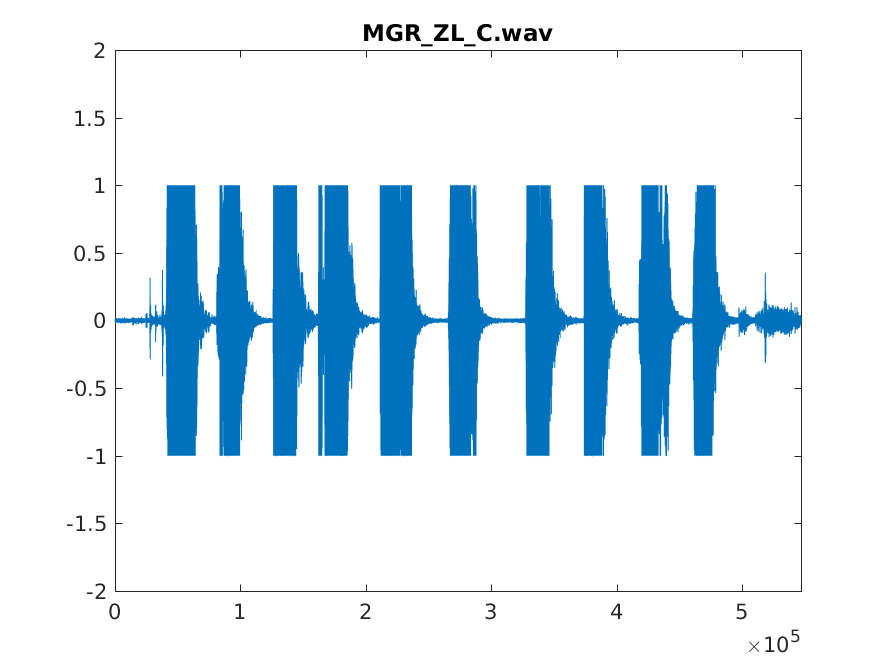
\includegraphics[width=\textwidth]{MGR_ZL_C-plot}
	\caption{Przykład ustandaryzowanego sygnału}
\end{figure}
\begin{figure}[h]
	\centering
	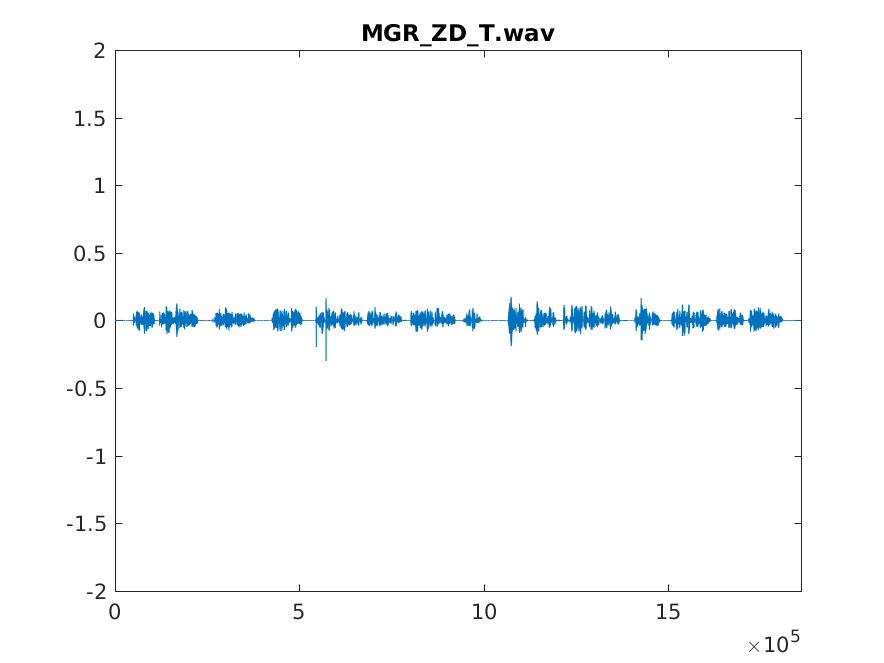
\includegraphics[width=\textwidth]{MGR_ZD_T-plot}
	\caption{Przykład nie ustandaryzowanego sygnału}
\end{figure}

Nagrania z korpusu nie były przetworzone wstępnie.
Poziom głośności nagrań różnił się pomiędzy nagraniami.
Zapis wypowiedzi został ustandaryzowany w celu zniwelowania różnic wynikających z głośności nagrania.
\section{}
\bibliography{praca_dyplomowa}{}
\bibliographystyle{plain}
\end{document}
%+++ END +++
